\documentclass{report}
\usepackage[utf8]{inputenc}
\usepackage[francais]{babel}
\usepackage{setspace}
\usepackage{graphicx}

\title{Cahier des charges: \\Projet Développement d'un dot-plot en html, javascript et webgl }
\author{Rania \bsc{Assab} \\ Aurélien \bsc{Luciani}\\ Quentin \bsc{Riché-Piotaix}\\ Mathieu \bsc{Schaeffer}}
\date{5 mars 2014}
\begin{document}

\maketitle

\tableofcontents
\addcontentsline{toc}{chapter}{Introduction}

\chapter*{Introduction}

Le Dotlet est une application disponible en ligne permettant de comparer deux séquences nucléotidiques ou protéiques en se basant sur la théorie du dot-plot. Cependant, pour pouvoir l'utiliser, il faut que la machine virtuelle Java soit installée sur la machine et disponible dans le navigateur.\\
L'objectif du projet est d'implémenter une interface web en utilisant les technologies standards actuelles, en ne nécessitant aucune extension navigateur et produisant le même type de résultat.\\
Ce logiciel a été codé par Marco Pagni et Thomas Junier, du Swiss Institute of Bioinformatics à Épalinges en Suisse. Jusqu'à présent, il n'y avait pas d'application permettant la comparaison de séquences à travers un navigateur web. Ils ont alors pris l'initiative de la faire et ont même continué son développement. En effet, la version 1.5 est sortie récemment avec plus de fonctionnalités.\\

\chapter{Dot-plot}

\section{Définition}

Le dot-plot est une des seules manières de comparer des séquences - nucléotidiques ou protéiques - pour mettre en évidence les séquences répétées ou palindromiques. C'est une technique remontant aux années 70 mais elle demeure efficace pour en avoir une vue générale.\\
Les éléments sont comparés deux à deux et les résultats de la comparaison sont illustrés par un graphique qui permet de mettre en évidence des zones d'intérêt.\\
De par la nature du dot-plot, la comparaison ne peut être effectuée qu'entre séquences de même type.\\

\section{Calculs des comparaisons et graphique}

Pour pouvoir interpréter les résultats, il faut comprendre comment se déroule le processus de comparaison. Par exemple, dans le cas de deux séquences de nucléotides : La première base de la première séquence est comparée avec la première base de la seconde séquence. Une matrice d'alignement de séquence doit être choisie pour l'analyse.\\
Son choix est important car selon la matrice choisie, le résultat sera différent. Les matrices doivent être sélectionnées selon les séquences à analyser car il en existe avec des pondérations différentes donnant des scores différents.\\
Pour représenter ceux-ci de manière ergonomique, à chaque score est associé un gradient de couleur, nous permettant de visualiser des motifs, comme des diagonales (cf fig.\ref{schema}). On peut alors en déduire la présence de similitudes ou de palindromes dans les séquences.\\


\begin{figure}[!h]
\centerline{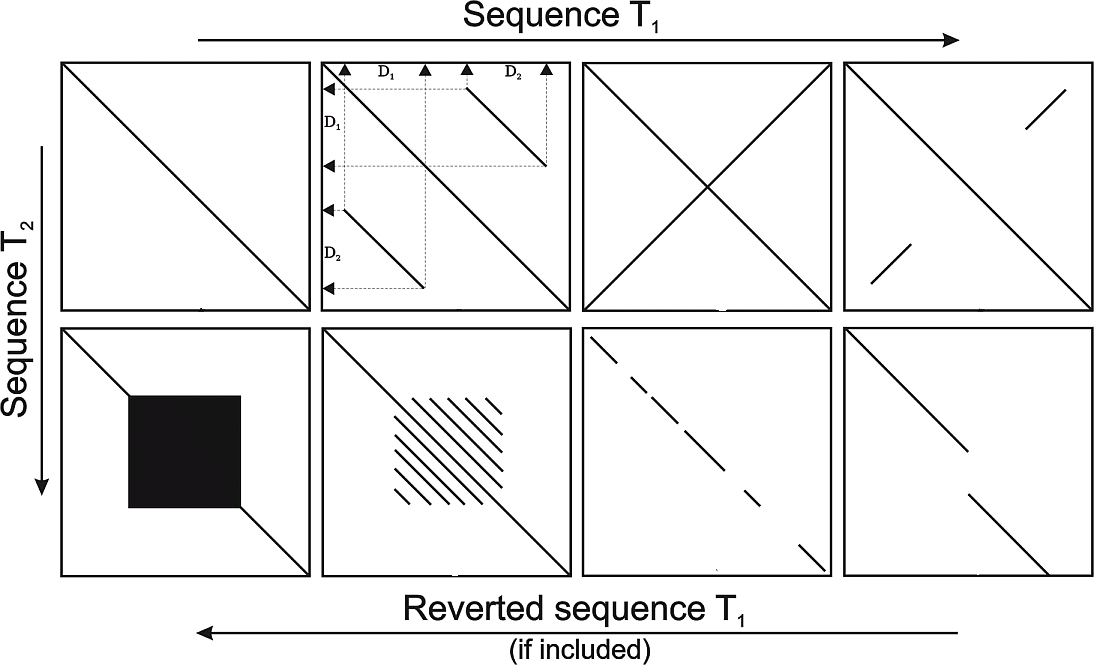
\includegraphics[scale=0.35]{SchemaDotplot.png}}
\caption{Représentation de différents résultats}
\label{schema}
\end{figure}

\chapter{Dotlet}
\section{Utilisation}

L'interface graphique permet la saisie des deux séquences à comparer. Elle s'effectue via copier-coller. Il est nécessaire de choisir une matrice d'alignement~: Identité (par défaut), BLOSUM, PAM, etc. Il est aussi possible de choisir une taille de fenêtre de comparaison et un zoom particuliers.\\
Les comparaisons peuvent se faire entre deux séquences d'ADN, deux protéines ou entre une séquence d'ADN et une séquence protéique. Dans ce dernier cas, l'ADN est traduit en séquence protéique par le biais des différents cadres de lecture possibles.\\

%publier les images du dotlet
\begin{figure}[!h]
\centering
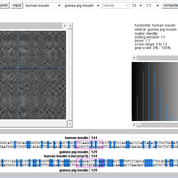
\includegraphics{image3.png}
Figure1: 
\end{figure}
\begin{figure}[!h]
\centering
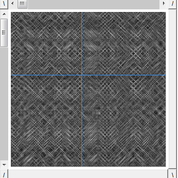
\includegraphics{image4.png}
Figure2:
\end{figure}
\begin{figure}[!h]
\centering
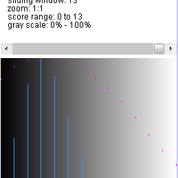
\includegraphics{image5.png}
Figure3:
\end{figure}
\begin{figure}[!h]
\centering
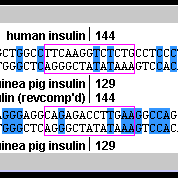
\includegraphics{image1.png}
Figure4:
\end{figure}

\chapter{Exigences}
\section{Besoins fonctionnels}
Selon les exigences données, il va falloir se conformer au Dotlet précédemment décrit.\\
Cet outil ayant été validé et utilisé pendant une dizaine d'années par de nombreux scientifiques, professeurs et étudiants, il représentera donc la référence.\\
L'objectif est d'en réaliser une version web plus accessible, utilisant les technologies HTML, WebGL et JavaScript. Celles-ci ayant évolué, il est maintenant possible de le faire sans utiliser Java et de ne plus dépendre d'un module externe.\\

\paragraph{Web} ~\\

Cet outil de dot-plot devra être disponible directement sur le web, cependant, le code devra être compatible avec les principaux navigateurs du marché.
Dans un premier temps, seuls les navigateurs Chrome et Firefox sont demandés.

\paragraph{Menu} ~\\

Tout d'abord, il va falloir réaliser un menu permettant d'initialiser les différents paramètres de ce dot-plot, incluant~:
\begin{itemize}
	\item L'enregistrement de séquences a comparer, via une entrée de texte.
	\item Le choix des 2 séquences dans une liste déroulante, parmi les séquences enregistrées.
	\item Le choix de la matrice de comparaison parmi celles récupérés dans la littérature.
	\item La taille de la fenêtre de comparaison, pour plus ou moins de précision dans notre dot-plot.
\end{itemize}

\paragraph{Graphe} ~\\
	L'affichage des résultats se fera sur un graphe traduisant les scores obtenus entre les 2 séquences, représentées en abscisse et en ordonnée. Ceux-ci sont représentés par un gradient de couleurs.\\
Chaque pixel de l'image représentera donc le score calculé selon la matrice et la taille de la fenêtre de comparaison passées en paramètres.

\paragraph{Fenêtre d'alignement} ~\\
	Une vision plus précise sera donnée par l'affichage d'une fenêtre d'alignement entre les 2 séquences.
Des ascenseurs permettront de naviguer sur celles-ci et de choisir une position pour chacune d'entre elle.\\
Devront y figurer la fenêtre de comparaison ainsi que le degré de similitude entre les éléments comparés.\\
D'autre part, certains cas particuliers devront être pris en compte.
Dans le cas où l'on étudierait le rapprochement entre une séquence d'ADN et une protéine, l'alignement comprendra la séquence protéique initiale, ainsi que les 3 séquences protéiques traduites des 3 cadres de lectures de la séquence nucléotidique.
Pour une comparaison entre ADN, les séquences seront comparées dans le même sens et dans des sens opposés.\\
Un clic sur l'image capturera les positions des séquences et l'alignement s'initialisera à partir de celles ci.

%Partir un jour, sans retour
\paragraph{Histogramme} ~\\

Enfin, un histogramme sera ajouté, mettant en évidence les pointes de gris correspondant aux scores affichés sur l'image.\\
Des ascenseurs permettront de faire fluctuer le contraste et de se focaliser uniquement sur certaines valeurs. Ces modifications  se répercuteront sur l'image, permettant de révéler des diagonales intéressantes, de pouvoir les sélectionner par un clic et de les afficher dans l'alignement.

\section{Besoins non fonctionnels}

\subsection{Fonctionnalités de la version 1.5}
Certaines fonctionnalités qui ne sont pas essentielles au bon déroulement de l'application ont été implémentée avec la version 1.5 du logiciel. Il s'agit de l'ajout d'un bouton permettant d'imprimer directement, qui pourra être remplacé par la possibilité de récupérer l'image. Les autres ajouts permettent, en combinant une action de la souris et une touche de clavier sélectionner zones d'intérêt dans l'image. Cela peut être une diagonale contenue dans la zone sélectionné si au moins la moitié des valeurs des points de cette diagonale dépassent un certain seuil (défini par l'utilisateur). Les séquences de ces diagonales peuvent ensuite être récupérées. C'est également le cas pour une autre fonctionnalité : l'utilisateur peut, en cliquant sur un point, récupérer la séquence de la diagonale sur laquelle il a cliqué, tant que les valeurs de cette diagonale sont au dessus du seuil qu'il a défini. Cette action peut être répétées, les séquences s'ajoutent. Enfin, le dernier ajout permet de voir facilement le positionnement dans les séquences avec un simple survol de la zone d'intérêt.

\subsection{Amélioration de certains points}
Quelques aspects de l'application Dotlet ne sont pas très satisfaisants et pourraient être améliorés pour donner plus de confort à l'utilisateur. Le zoom notamment, la façon de faire est peu intuitive, et il serait préférable d'utiliser la molette de la souris. L'autre point important est la gestion de la traduction : en effet, on peut choisir de comparer une séquence nucléotidique a une séquence protéique, mais en raison des multiples cadres de lectures, le calcul repose sur une moyenne avec une seuil adapté. Une solution pourrait être de ne s'occuper que de la séquence protéique la plus longue des trois cadres de lectures. En effet, la séquence la plus longue disponible est probablement la séquence d'intérêt. Enfin, l'interface pourrait gagner en esthétisme et surtout et ergonomisme.

\section{Test du programme}

30 mars, L3 ?
Jeu de données

\chapter{Environnement de Programmation}

Dans le cadre de ce projet, plusieurs langages seront utilisés. Les langages HTML/CSS serviront à structurer l'affichage dans les navigateurs web. L'interface WebGL améliorera l'affichage sur l'écran. Contrairement aux auteurs du dotlet, le développement du dot-plot sera codé en JavaScript.  Ce dernier langage est nécessaire pour utiliser WebGL.


\chapter{Architecture}
Utilisation des langages
Maquette ?

Aurélien


\chapter{Planning previsionnel}
almost done



\addcontentsline{toc}{chapter}{Conclusion}
\chapter*{Conclusion et perspectives}


\addcontentsline{toc}{chapter}{Références}
\chapter*{Références}
Le site du dotlet: http://myhits.isb-sib.ch/cgi-bin/dotlet\\
L'article des auteurs du dotlet, Thomas Junier et Marco Pagni: http://bioinformatics.oxfordjournals.org/content/16/2/178.long\\



\end{document}
